\documentclass[11pt]{article}
\usepackage{graphicx}
\raggedbottom
\author{}
\date{}
\title{Esempio della regressione lineare usando l'andamento del prezzo degli stock di nvidia\vspace*{-3em}}
\begin{document}
\maketitle
\section*{Cenni teorici}
La regressione lineare è un metodo statistico utilizzato per modellare la relazione tra una variabile dipendente
\textbf{Y} (detta anche risposta o output) e una o più variabili indipendenti 
\textbf{X} (dette anche predittori o input). Lo scopo principale è stimare una funzione lineare che descriva come \textbf{Y} 
varia al variare di \textbf{X}.
\\Nel caso più semplice (regressione lineare semplice, con una sola variabile indipendente), il modello si esprime come:
\begin{equation}
    Y=\beta_0+\beta_1*X+\varepsilon  
\end{equation}
\begin{itemize}
    \item \textbf{Y}:variabile dipendente.
    \item \textbf{X}:variabile indipendente.
    \item \begin{math}\mathbf{\beta_0}\end{math}:intercetta (il valore previsto di \textbf{Y}quando \textbf{X}=0).
    \item \begin{math} \mathbf{\beta_1}\end{math}:coefficiente angolare (indica quanto cambia \textbf{Y} per ogni unità
          di incremento in \textbf{X}).
    \item \begin{math}\mathbf{\varepsilon}\end{math}:termine di errore, che rappresenta la differenza
          tra il valore osservato e quello previsto dal modello.       
\end{itemize}
Quando analizziamo i dati finanziari di una società, come i prezzi di mercato delle azioni, possiamo utilizzare tecniche statistiche come la regressione lineare per studiare 
le relazioni tra variabili rilevanti. Questa tecnica permette di modellare matematicamente una variabile 
dipendente (ad esempio, il prezzo di mercato) in funzione di variabili indipendenti (ad esempio, utili per azione o volumi di scambio).
\newpage
\begin{center}
    Esempi:\\

\begin{figure}[ht!]
    \centering
    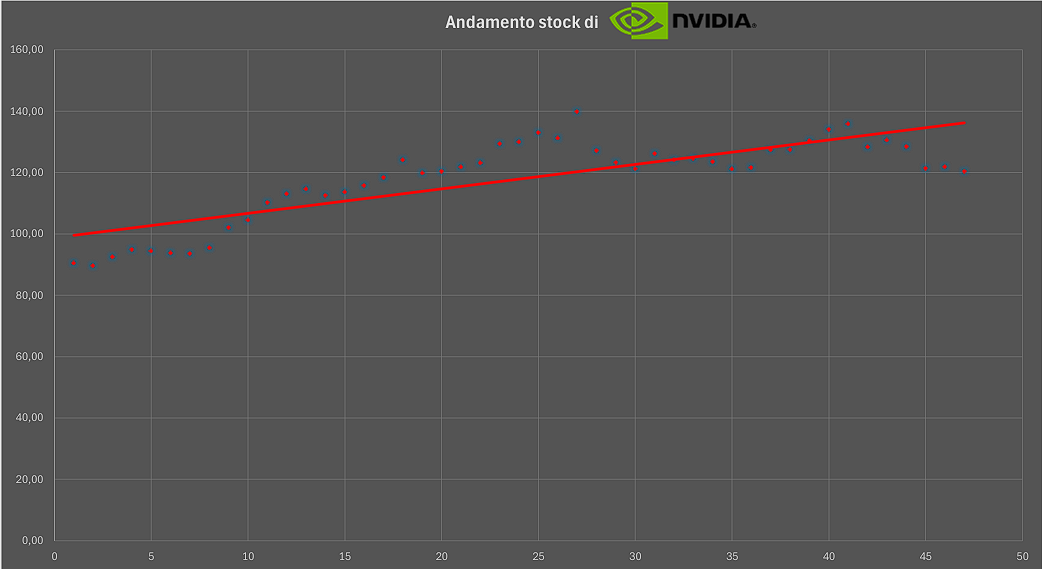
\includegraphics[width=\textwidth]{immagini/Screenshot 2024-11-20 000800.png}
    \caption{in questo esempio possiamo vedere l'andamento del prezzo degli stock di nvidia in base alla data con un campione di dati di 2 mesi.}
\end{figure}
%n questo esempio possiamo vedere l'andamento del prezzo degli stock di nvidia in base alla data con un campione di dati di 2 mesi.\\
\begin{figure}[ht!]
    \centering
    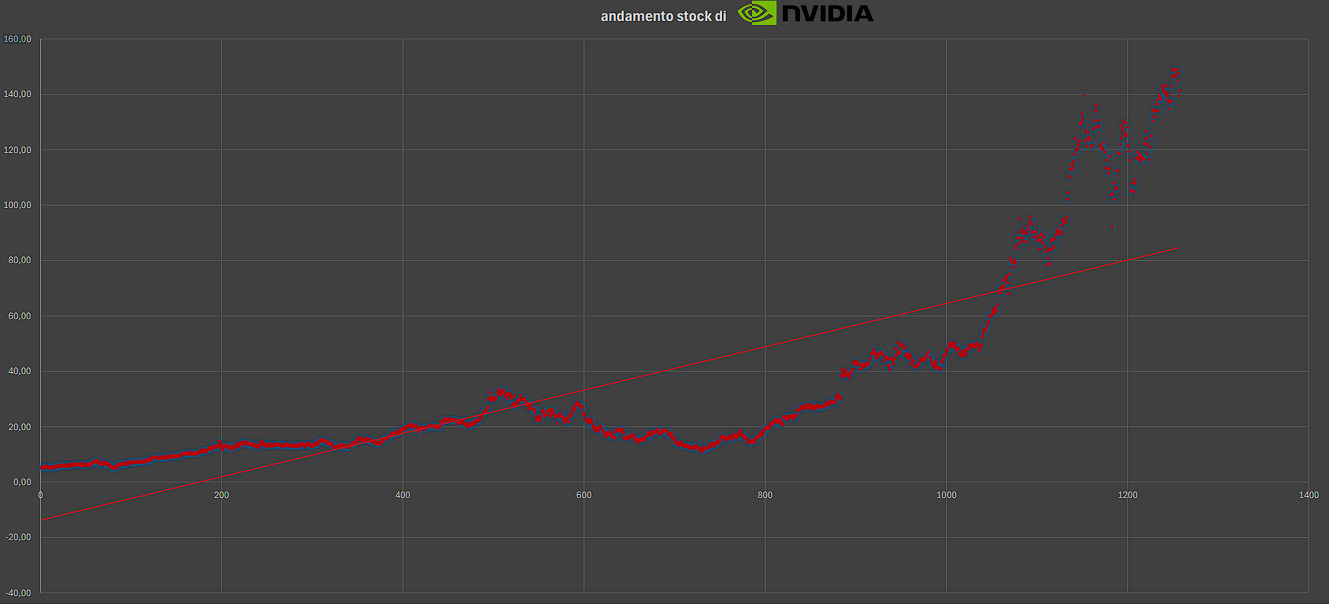
\includegraphics[width=\textwidth]{immagini/Screenshot 2024-11-20 210756.png}
    \caption{Mentre in questo esempio possiamo vedere l'andamento del prezzo degli stock di nvidia in base alla data con un campione di dati di 5 anni.}
\end{figure}
%Mentre in questo esempio possiamo vedere l'andamento del prezzo degli stock di nvidia in base alla data con un campione di dati di 5 anni.
\end{center}
\section*{Conclusione:}
La regressione lineare è un metodo per analizzare relazioni tra variabili e fare previsioni. Viene usata in economia, ingegneria, medicina, ambiente e finanza 
per stimare cambiamenti e comprendere fenomeni. Il modello lineare consente di identificare come una variabile dipende da un'altra. È semplice, versatile e applicabile 
in molti ambiti.
\end{document}